%\documentclass{beamer}
\documentclass[handout]{beamer}
\usepackage[francais]{babel}
\usepackage[utf8]{inputenc}
\usepackage[T1]{fontenc}
\usepackage{dcolumn}
\usepackage{graphicx}
\usepackage{epsfig}
\usepackage{pgf}
\usepackage{pstricks}
\usepackage{pst-node}
\usepackage{listings}
\newcolumntype{.}{D{.}{.}{-1}}
\newcolumntype{d}[1]{D{.}{.}{#1}}
\usetheme{Malmoe}

\setbeamertemplate{frametitle}[default][center]
\beamerdefaultoverlayspecification{<+->}

\lstdefinelanguage{Coq}{ 
%
% Anything betweeen $ becomes LaTeX math mode
mathescape=true,
texcl=false, 
%
% Vernacular commands
morekeywords=[1]{Section, Module, End, Require, Import, Export,
  Variable, Variables, Parameter, Parameters, Axiom, Hypothesis,
  Hypotheses, Notation, Local, Tactic, Reserved, Scope, Open, Close,
  Bind, Delimit, Definition, Let, Ltac, Fixpoint, CoFixpoint, Add,
  Morphism, Relation, Implicit, Arguments, Unset, Contextual,
  Strict, Prenex, Implicits, Inductive, CoInductive, Record,
  Structure, Canonical, Coercion, Context, Class, Global, Instance,
  Program, Infix, Theorem, Lemma, Corollary, Proposition, Fact,
  Remark, Example, Proof, Goal, Save, Qed, Defined, Hint, Resolve,
  Rewrite, View, Search, Show, Print, Printing, All, Eval, Check,
  Projections, inside, outside, Def},
%
% Gallina
morekeywords=[2]{forall, exists, exists2, fun, fix, cofix, struct,
  match, with, end, as, in, return, let, if, is, then, else, for, of,
  nosimpl, when},
%
% Sorts
morekeywords=[3]{Type, Prop, Set, true, false, option},
%
% Various tactics, some are std Coq subsumed by ssr, for the manual purpose
morekeywords=[4]{pose, set, move, case, elim, apply, clear, hnf,
  intro, intros, generalize, rename, pattern, after, destruct,
  induction, using, refine, inversion, injection, rewrite, congr,
  unlock, compute, ring, field, fourier, replace, fold, unfold,
  change, cutrewrite, simpl, have, suff, wlog, suffices, without,
  loss, nat_norm, assert, cut, trivial, revert, bool_congr, nat_congr,
  symmetry, transitivity, auto, split, left, right, autorewrite},
%
% Terminators
morekeywords=[5]{by, done, exact, reflexivity, tauto, romega, omega,
  assumption, solve, contradiction, discriminate},
%
% Control
morekeywords=[6]{do, last, first, try, idtac, repeat},
%
% Comments delimiters, we do turn this off for the manual
morecomment=[s]{(*}{*)},
%
% Spaces are not displayed as a special character
showstringspaces=false,
%
% String delimiters
morestring=[b]",
morestring=[d]�,
%
% Size of tabulations
tabsize=2,
%
% Enables ASCII chars 128 to 255
extendedchars=false,
%
% Case sensitivity
sensitive=true,
%
% Automatic breaking of long lines
breaklines=false,
%
% Default style fors listings
basicstyle=\small,
%
% Position of captions is bottom
captionpos=b,
%
% flexible columns
columns=[l]flexible,
%
% Style for (listings') identifiers
identifierstyle={\ttfamily\color{black}},
% Style for declaration keywords
keywordstyle=[1]{\ttfamily\color{violet}},
% Style for gallina keywords
keywordstyle=[2]{\ttfamily\color{green!80!black}},
% Style for sorts keywords
keywordstyle=[3]{\ttfamily\color{cyan}},
% Style for tactics keywords
keywordstyle=[4]{\ttfamily\color{blue}},
% Style for terminators keywords
keywordstyle=[5]{\ttfamily\color{red}},
%Style for iterators
%keywordstyle=[6]{\ttfamily\color{dkpink}},
% Style for strings
stringstyle=\ttfamily,
% Style for comments
commentstyle={\ttfamily\color{red!50!black}},
%
%moredelim=**[is][\ttfamily\color{red}]{/&}{&/},
literate=
    {\\forall}{{\color{green!80!black}{$\forall\;$}}}1
    {\\exists}{{$\exists\;$}}1
    {<-}{{$\leftarrow\;$}}1
    {=>}{{$\Rightarrow\;$}}1
    %{==}{{\code{==}\;}}1
    {==>}{{\code{==>}\;}}1
%    {:>}{{\code{:>}\;}}1
    {->}{{$\rightarrow\;$}}1
    {<->}{{$\leftrightarrow\;$}}1
    {<==}{{$\leq\;$}}1
    {\#}{{$^\star$}}1 
    {\\o}{{$\circ\;$}}1 
    {\@}{{$\cdot$}}1 
    {\/\\}{{$\wedge\;$}}1
    {\\\/}{{$\vee\;$}}1
    %{++}{{\code{++}}}1
    {~}{{\ }}1
    {\@\@}{{$@$}}1
    {\\mapsto}{{$\mapsto\;$}}1
    {\\hline}{{\rule{\linewidth}{0.5pt}}}1
%
}[keywords,comments,strings]

\definecolor{mygrey}{rgb}{0.91,0.90,0.90}
\lstset{language=Coq,backgroundcolor=\color{mygrey}}

\title{Soutenance de Stage}
\author{Arthur Wenger \& Karim Mamode}
\date{03 Juin 2017}
\institute{\normalsize{L3 Informatique Université de la Réunion}}
\begin{document}

\begin{frame}
  \titlepage
\end{frame}

\begin{frame}
  \frametitle<1->{\center{Introduction}}
  \begin{block}<1->{Objectifs}
    \begin{itemize}
    \item <1->{Analyser un protocole de routage expérimental}
    \item <2->{Modéliser un réseau}
    \item <3->{Prouver des propriétés du réseau à travers la modélisation}
    \end{itemize}
  \end{block}
    \begin{block}<2->{Outils}
    \begin{itemize}
    \item <4->{Le logiciel Coq pour l'élaboration de preuves}
    \item <5->{Le langage de programmation fonctionnel Gallina}
    \end{itemize}
  \end{block}
\end{frame}

\begin{frame}
  \frametitle<1->{\center{Analyse et Modélisation}}
\begin{block}<1->{Analyse du protocole}
    \begin{itemize}
    \item <1->{Diviser le réseau en régions}
    \item <2->{Aggréger les informations sur les noeuds d'une région}
    \item <3->{Créer des routes vers des noeuds et des régions}
    \item <4->{Appliquer un algorithme pour remplir les tables de routage}
    \end{itemize}
  \end{block}
  \begin{block}<2->{Modélisation}
    \begin{itemize}
    \item <5->{Modéliser une région}
    \item <6->{Réprésenter la structure des régions dans le réseau}
    \item <7->{Décrire les liens entre les noeuds du réseau}
    \item <8->{Représenter une route et un chemin entre deux noeuds}
    \end{itemize}
  \end{block}
\end{frame}

\begin{frame}[fragile]
  \frametitle<1->{\center{Les Régions}}
    \begin{itemize}
    \item <1->{Un type inductif pour le codage des régions}
      \begin{lstlisting}
      Inductive region : Type :=
      | Z : region
      | OO : region -> region
      | OI : region -> region
      | II : region -> region
      | IO : region -> region.
      \end{lstlisting}
    \item <2->{Un codage comparable à la base 4}
    \item <3->{Permet de représenter l'imbrication des régions}%Regions mères/filles
    \item <4->{Un élément neutre pour le type inductif: Z}
    \end{itemize}
\end{frame}

\begin{frame}
  \frametitle<1->{\center{Interactions entre les régions}}
    \begin{block}<1->{Objectifs}
    \begin{itemize}
    \item <1->{Représenter la structure des régions dans le réseau}
    \item <2->{Définir la notion de régions voisines}
    \item <3->{Calculer les distances entre les régions}
    \end{itemize}
  \end{block}
  \begin{block}<2->{Moyens}
    \begin{itemize}
    \item <4->{Listes de régions}
    \item <5->{Matrices de régions}
    \item <6->{Algorithme de partionnement du réseau}
    \end{itemize}
  \end{block}
\end{frame}

\begin{frame}[fragile]
  \frametitle<1->{\center{Listes}}

    \begin{itemize}
    \item <1->{Un type inductif polymorphe pour représenter des listes}
    \begin{lstlisting}
    Inductive clist (A:Type): Type :=
      | nil : clist A
      | cons : A -> clist A -> clist A.
    \end{lstlisting}
    \item <2->{Interprétée comme un vecteur pour la construction de matrices}
    \item <2->{Pas de contraintes sur le nombre d'élements}
    \end{itemize}
\end{frame}

\begin{frame}[fragile]
  \frametitle<1->{\center{Listes de listes}}
    \begin{itemize}
    \item <1->{Un type inductif polymorphe pour représenter des listes de listes}
    \begin{lstlisting}
    Inductive listlist (A:Type) : Type :=
      | lnil : listlist A
      | lcons : clist A -> listlist A -> listlist A.
    \end{lstlisting}
    \item <2->{Pas nécessairement homogènes}
    \item <3->{Un ensemble englobant les matrices}
    \item <4->{Pas de contraintes sur le nombres de listes}
    \end{itemize}
\end{frame}

\begin{frame}[fragile]
  \frametitle<1->{\center{Matrices}}
    \begin{itemize}
    \item <1->{Un sous ensemble des listes de listes}
    \item <1->{Nécessité de vérifier qu'une liste de listes est une matrice}%2ème possibilité = intégrer une hypothèse dans les paramètres du constructeur
    \begin{lstlisting}
    Fixpoint is_matrix {A:Type}(m:listlist A) : bool :=
      match m with
      | lnil => true
      | lcons l m' => 
            match m' with
            | lnil => true
            | lcons l' m'' => Nat.eqb (list_count l) 
                                      (list_count l')
                               && is_matrix m'
              end
      end.
    \end{lstlisting}%2ème version?
    \end{itemize}
\end{frame}

\begin{frame}[fragile]
  \frametitle<1->{\center{Matrices carrées}}
    \begin{itemize}
    \item <1->{Un sous ensemble des matrices}
    \item <1->{Permet de représenter le partionnement du réseau}
    \begin{lstlisting}
  Definition is_square_matrix {A:Type}(m:listlist A): 
  bool :=
  match m with
  | lnil => true
  | lcons l' m' => (is_matrix m) && (Nat.eqb (list_count l') 
                                               (mat_count m))
  end.
    \end{lstlisting}%pas de constructeur propre pour les matrices
    \end{itemize}
\end{frame}

\begin{frame}
  \frametitle<1->{Partitionnement du réseau}
    \begin{itemize}
    \item <1->{Représenter l'organisation des régions sous forme matricielle}
    \begin{center}
    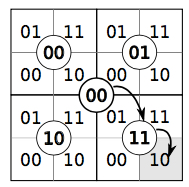
\includegraphics[width=40mm]{Sous_region.jpg}
    \end{center}
    \item <2->{Implémentation des partitionnements bottom-up et top-down}%définir les approches / prouver que les 2 approches sont possibles
    \item <3->{Chaque région de la matrice finale a un numéro global}%donc unique
    \item <4->{Notion de distance entre 2 régions pour un niveau donné}
    \end{itemize}
\end{frame}

\begin{frame}
  \frametitle<1->{Réseau}
    \begin{itemize}
    \item <1->{On cherche à représenter le graphe réseau}
    \begin{center}
    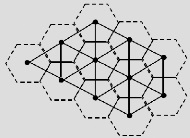
\includegraphics[width=40mm]{graph.jpg}
    \end{center}
    \item <2->{Représenter les liens entre les noeuds}
    \item <3->{Modéliser un chemin entre 2 noeuds}
    \item <4->{Définir les relations entre les noeuds et les régions}
    \end{itemize}
\end{frame}

\begin{frame}[fragile]
  \frametitle<1->{Noeuds et Chemins}
    \begin{itemize}
    \item <1->{Un noeud est identifié par un entier}
    \item <2->{Les liens sont modélisés par une fonction booléenne sur une paire de noeuds}
    \begin{lstlisting}
    Definition netnode := nat.
    Definition graph:= netnode -> netnode -> bool.
    \end{lstlisting}
    \item <3->{En ajoutant la propriété de transitivité on définit des chemins }
    \begin{lstlisting}
  Inductive has_path (g:graph) : nat -> netnode -> netnode -> 
  Prop :=
  | HP_Self (x:netnode): has_path g O x x 
  | HP_Step (n:nat) 
            (x y z:netnode) 
            (ST: g x y = true) 
            (HP: has_path g n y z): has_path g (S n) x z.
    \end{lstlisting}
    \end{itemize}
\end{frame}

\begin{frame}[fragile]
  \frametitle<1->{Localisation}
    \begin{itemize}
    \item <1->{Définir l'appartenance d'un noeud à une region}
    \begin{lstlisting}
    Definition loc_geo := region -> netnode -> bool.
    \end{lstlisting}
    \item <2->{Modéliser les paramètres "k" et "m" du protocole}
    \item <3->{Définir les contraintes}%chaque noeud appartient à une region par exemple
    \begin{lstlisting}
forall (x:netnode) (l:loc_geo), { r : region | l r x = true /\ 
                                               rank r = m }.
    \end{lstlisting}%parler des regions disjointes/imbriquées
    \item <3->{Deux noeuds sont-ils dans A0 ?}
    \begin{lstlisting}
Definition is_in_A0 (r1 r2:region)(m: listlist region): 
bool := 
match distance_regions_elem r1 r2 m with
| None => false
| Some d => d <? k
end.
    \end{lstlisting}    
    \end{itemize}
\end{frame}

\begin{frame}[fragile]
  \frametitle<1->{Routes et Tables}
    \begin{itemize}
    \item <1->{Un ensemble de destinations vers des noeuds ou des régions}
       \begin{lstlisting}
Inductive table (l:loc_geo)(m: listlist region)(x:netnode): 
Set :=
| rA0: ... (* l'ensemble des noeuds du reseau 
               situes dans A0 par rapport a x *)
| rAn: ... (* l'ensemble des regions voisines 
               de la region elementaire contenant x *)
    \end{lstlisting} 
    \item <2->{Le coût n'est pas représenté pour simplifier les premières preuves }
   \end{itemize}
\end{frame}

\begin{frame}
  \frametitle<1->{Preuves}
    \begin{itemize}
    \item <1->{Necessité d'itérer sur les étapes du cheminement d'un message}
    \item <2->{Mesurer les variations de distances vers la destination}
    \item <3->{Modéliser l'algorithme de contournement des vides}
    \item <4->{Montrer qu'il ne peut pas y avoir de boucle réseau}
    \item <5->{Montrer qu'il existe toujours des valeurs de k et de m qui 
    permettent de trouver le chemin menant vers une destination}
   \end{itemize}
\end{frame}

\end{document}
